\documentclass[a4paper]{article}

\usepackage[english]{babel}
\usepackage[utf8]{inputenc}
\usepackage{amsmath}
\usepackage{graphicx}
\usepackage[colorinlistoftodos]{todonotes}
\usepackage{hyperref}

\title{Capstone Project for Udacity Machine Learning Nanodegree}

\author{Pär Steffansson}

\date{\today}

\begin{document}
\maketitle

\begin{abstract}
I selected the competition \href{https://www.kaggle.com/c/zillow-prize-1#description}{Zillow Prize} found at
\href{https://www.kaggle.com}{Kaggle} as the Capstone project in my \textit{Machine Learning Engineer Nanodegree}
provided by \href{https://www.udacity.com}{Udacity}.
\end{abstract}

\tableofcontents

\section{Project Definition}
An overview of the project definition is described below. For more details see the competition
\href{https://www.kaggle.com/c/zillow-prize-1#description}{Zillow Prize}.

\subsection{Project Overview}
%
% Student provides a high-level overview of the project in layman’s terms. Background information such as the
% problem domain, the project origin, and related data sets or input data is given.
%
I selected the competition \href{https://www.kaggle.com/c/zillow-prize-1#description}{Zillow Prize} found at
\href{https://www.kaggle.com}{Kaggle} as the Capstone project in my \textit{Machine Learning Engineer Nanodegree}
provided by \href{https://www.udacity.com}{Udacity}.

\href{https://www.zillow.com}{Zillow} is the leading real estate and rental marketplace dedicated to empowering
consumers with data. They launched the Kaggle competition \textit{Zillow Prize} to improve their ability to predict
house prices.

I selected this competition to learn from the rich source of knowledge the community around these competitions
provide. Comparing and learning from public Kernels provided gives a good benchmark of cutting edge models
for these kind of problems.

\subsection{Problem Statement}
%
% The problem which needs to be solved is clearly defined. A strategy for solving the problem, including discussion
% of the expected solution, has been made.
%
They have been developing their own model to predict prices for years. The problem at hand is to see if the
Kaggle community can improve on it creating an even better model.

\subsection{Metrics}
%
% Metrics used to measure performance of a model or result are clearly defined. Metrics are justified based on the
% characteristics of the problem.
%
The metric is defined by Zillow witch is asking to predict the \textit{logerror} between their Zestimate model and the
actual sale price, given all the features of a home. The log error is defined as
\[ logerror = log(Zestimate) - log(SalePrice) \]
% TODO: Define the accual matric to use when models are learning


\section{Analysis}

\subsection{Data Exploration}
% If a dataset is present, features and calculated statistics relevant to the problem have been reported and
% discussed, along with a sampling of the data. In lieu of a dataset, a thorough description of the input space or
% input data has been made. Abnormalities or characteristics about the data or input that need to be addressed
% have been identified.
% Exploratory Visualization
% A visualization has been provided that summarizes or extracts a relevant characteristic or feature about the dataset
% or input data with thorough discussion. Visual cues are clearly defined.
This data exploration is inspired by the
\href{https://www.kaggle.com/sudalairajkumar/simple-exploration-notebook-zillow-prize}{Simple Exploration Notebook - Zillow Prize}
written by Kaggle Grandmaster \href{https://www.kaggle.com/sudalairajkumar}{SRK}.

We will be working with following data files
\begin{itemize}
    \item \textit{properties\_2016.csv} - all the properties with their home features for 2016. Note: Some 2017 new 
    properties don't have any data yet except for their parcelid's. Those data points should be populated when
    properties\_2017.csv is available.
    \item \textit{train\_2016.csv} - the training set with transactions from 1/1/2016 to 12/31/2016.
    \item \textit{sample\_submission.csv} - a sample submission file in the correct format
\end{itemize}

\subsubsection{Traning Set File}
The training set in file \textit{train\_2016.csv} contains 90275 rows and three columns
\begin{itemize}
    \item \textit{parcelid} - which is the id of the property.
    \item \textit{logerror} - the log-error comparing the log of the actual price and the log of the predicted price.
    \item \textit{transactiondate} - is the date when the property was sold
\end{itemize}

Each row correspond to a property transaction and there will be more than one row in this file with the same
parcelid if the property has been sold more than ones during 2016. In fact counting there are
\begin{itemize}
    \item 90026 properties that have been sold ones
    \item 123 properties that have been sold twice
    \item and one property that was sold one time.
\end{itemize}

\begin{figure}
\centering
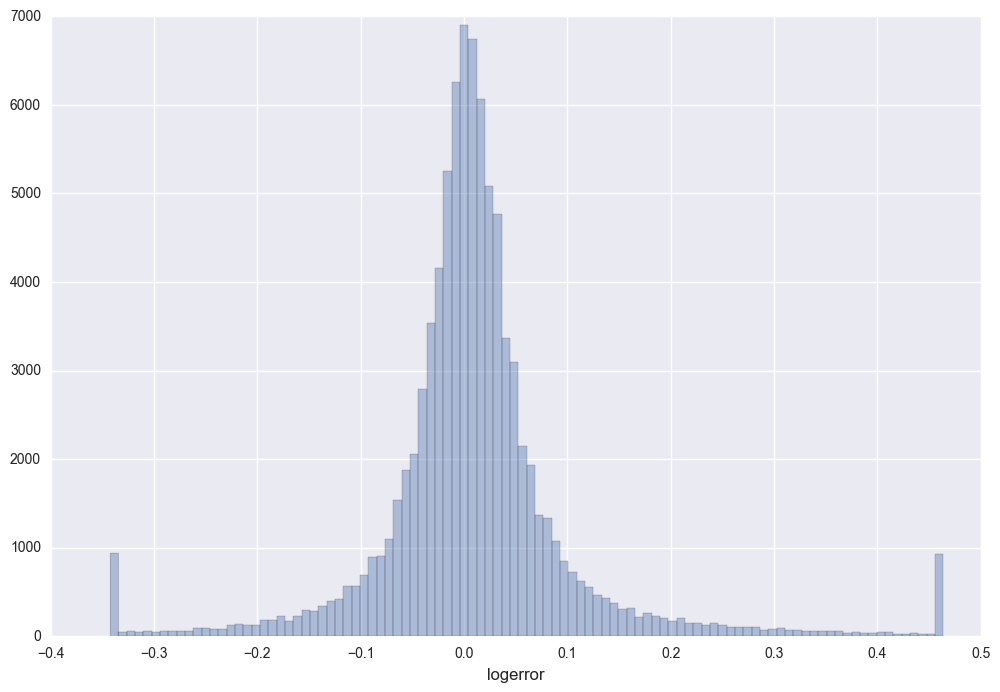
\includegraphics[width=1\textwidth]{./img/train-logerror.png}
\caption{\label{fig:logerror}Logerror distribution}
\end{figure}
Looking at Figure \ref{fig:logerror} the log error has nice normal distribution centered around zero.

\begin{figure}
\centering
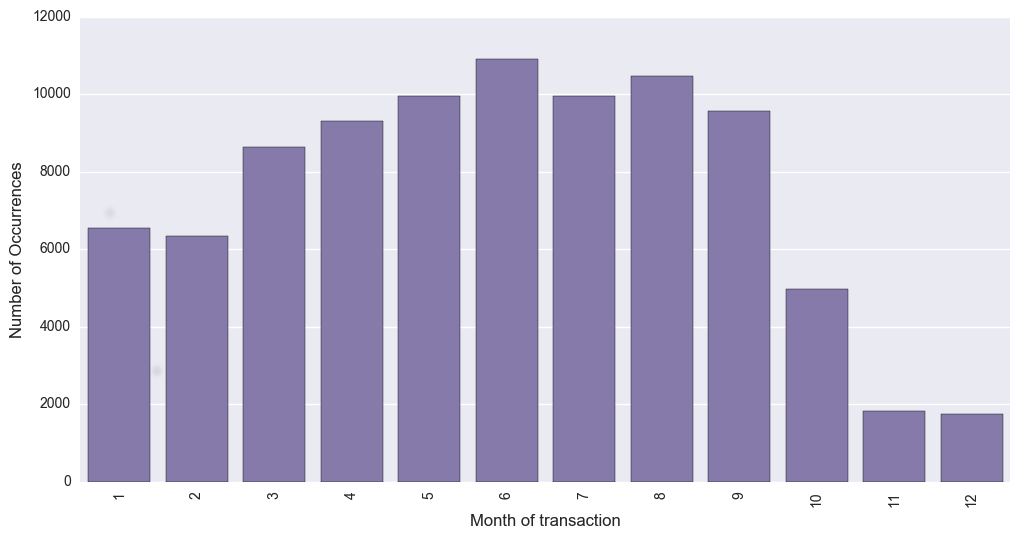
\includegraphics[width=1\textwidth]{./img/train-transactiondate.png}
\caption{\label{fig:transactions}Number of transactions over time}
\end{figure}
According to Zillow the training data has all the transactions before October 15, 2016, plus some of the transactions
after October 15, 2016. Looking at Figure \ref{fig:transactions} from January to September there are about 6000-11000
transactions per month while dropping to under 2000 in November to December.

\subsubsection{Properties}
Property data file \textit{properties\_2016.csv} is a lot larger with 2985217 rows and 58 columns describing home
features. It seems like some of the columns contain less information in the form of NaN values.
\begin{figure}
\centering
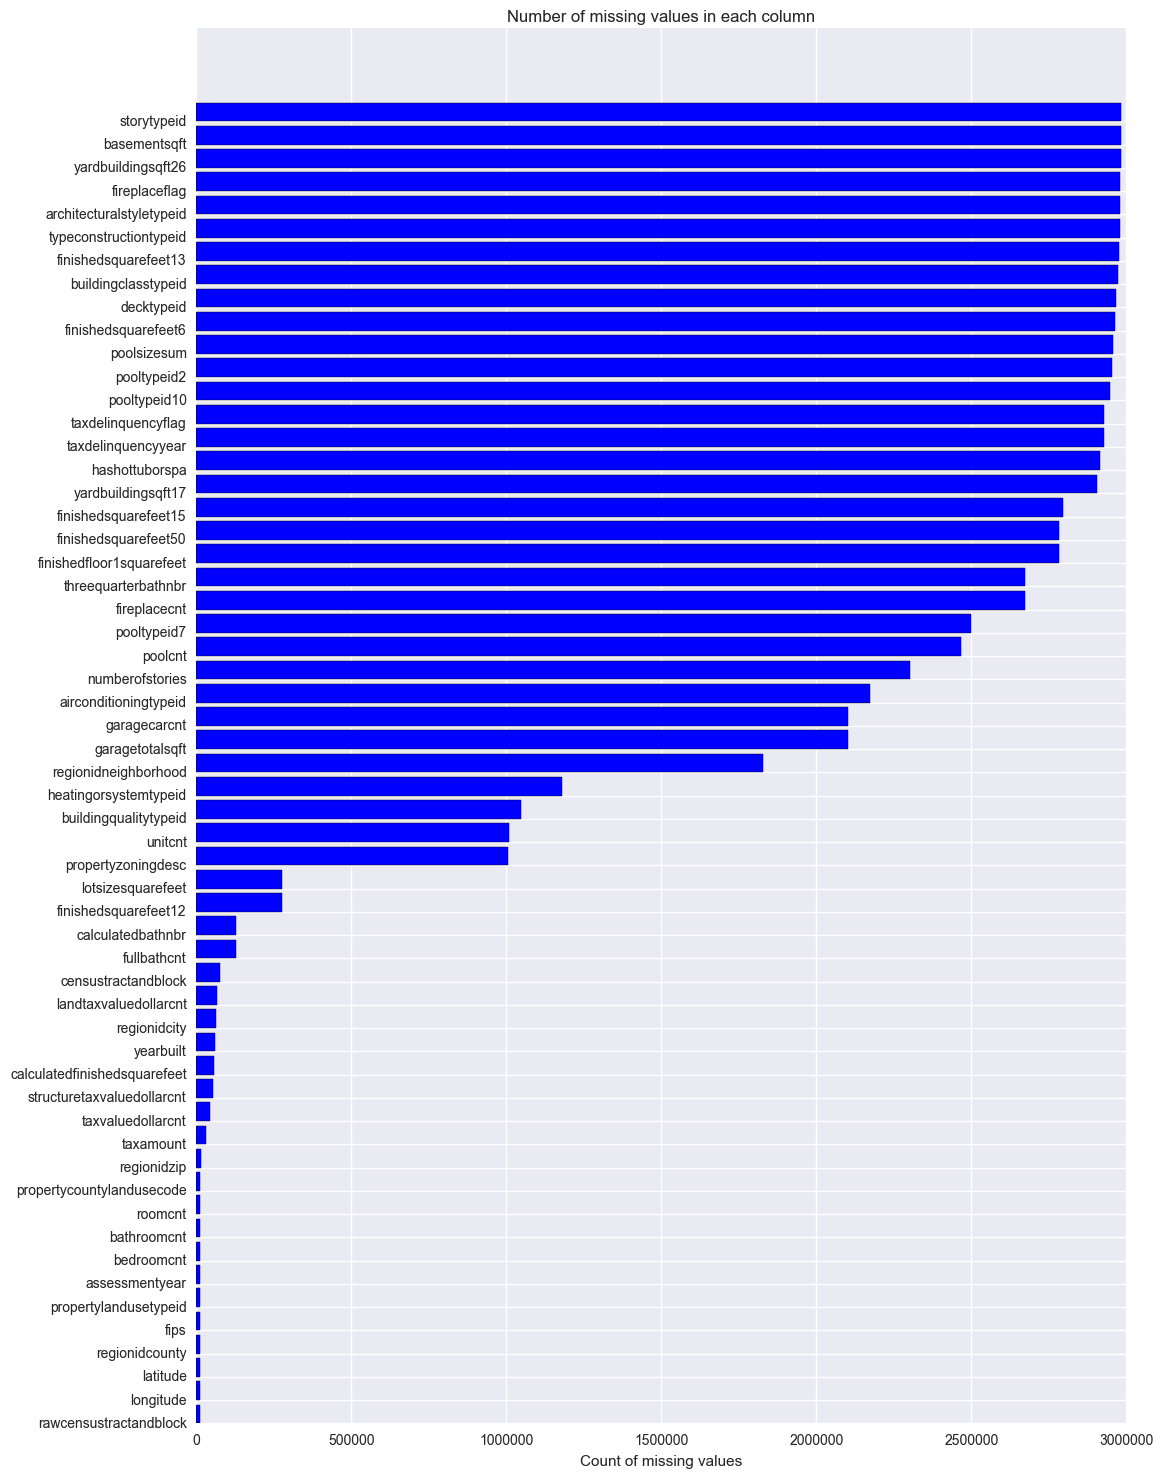
\includegraphics[width=1\textwidth]{./img/prop-nan.png}
\caption{\label{fig:prop-nan} Amount of information in features}
\end{figure}
Looking at Figure \ref{fig:prop-nan} more than half of the data is not there and the
data loss is unevenly distribute on featues. About 30 percent of the features will
most likely not contribute to a better model when they do not contain any information.

\begin{figure}
\centering
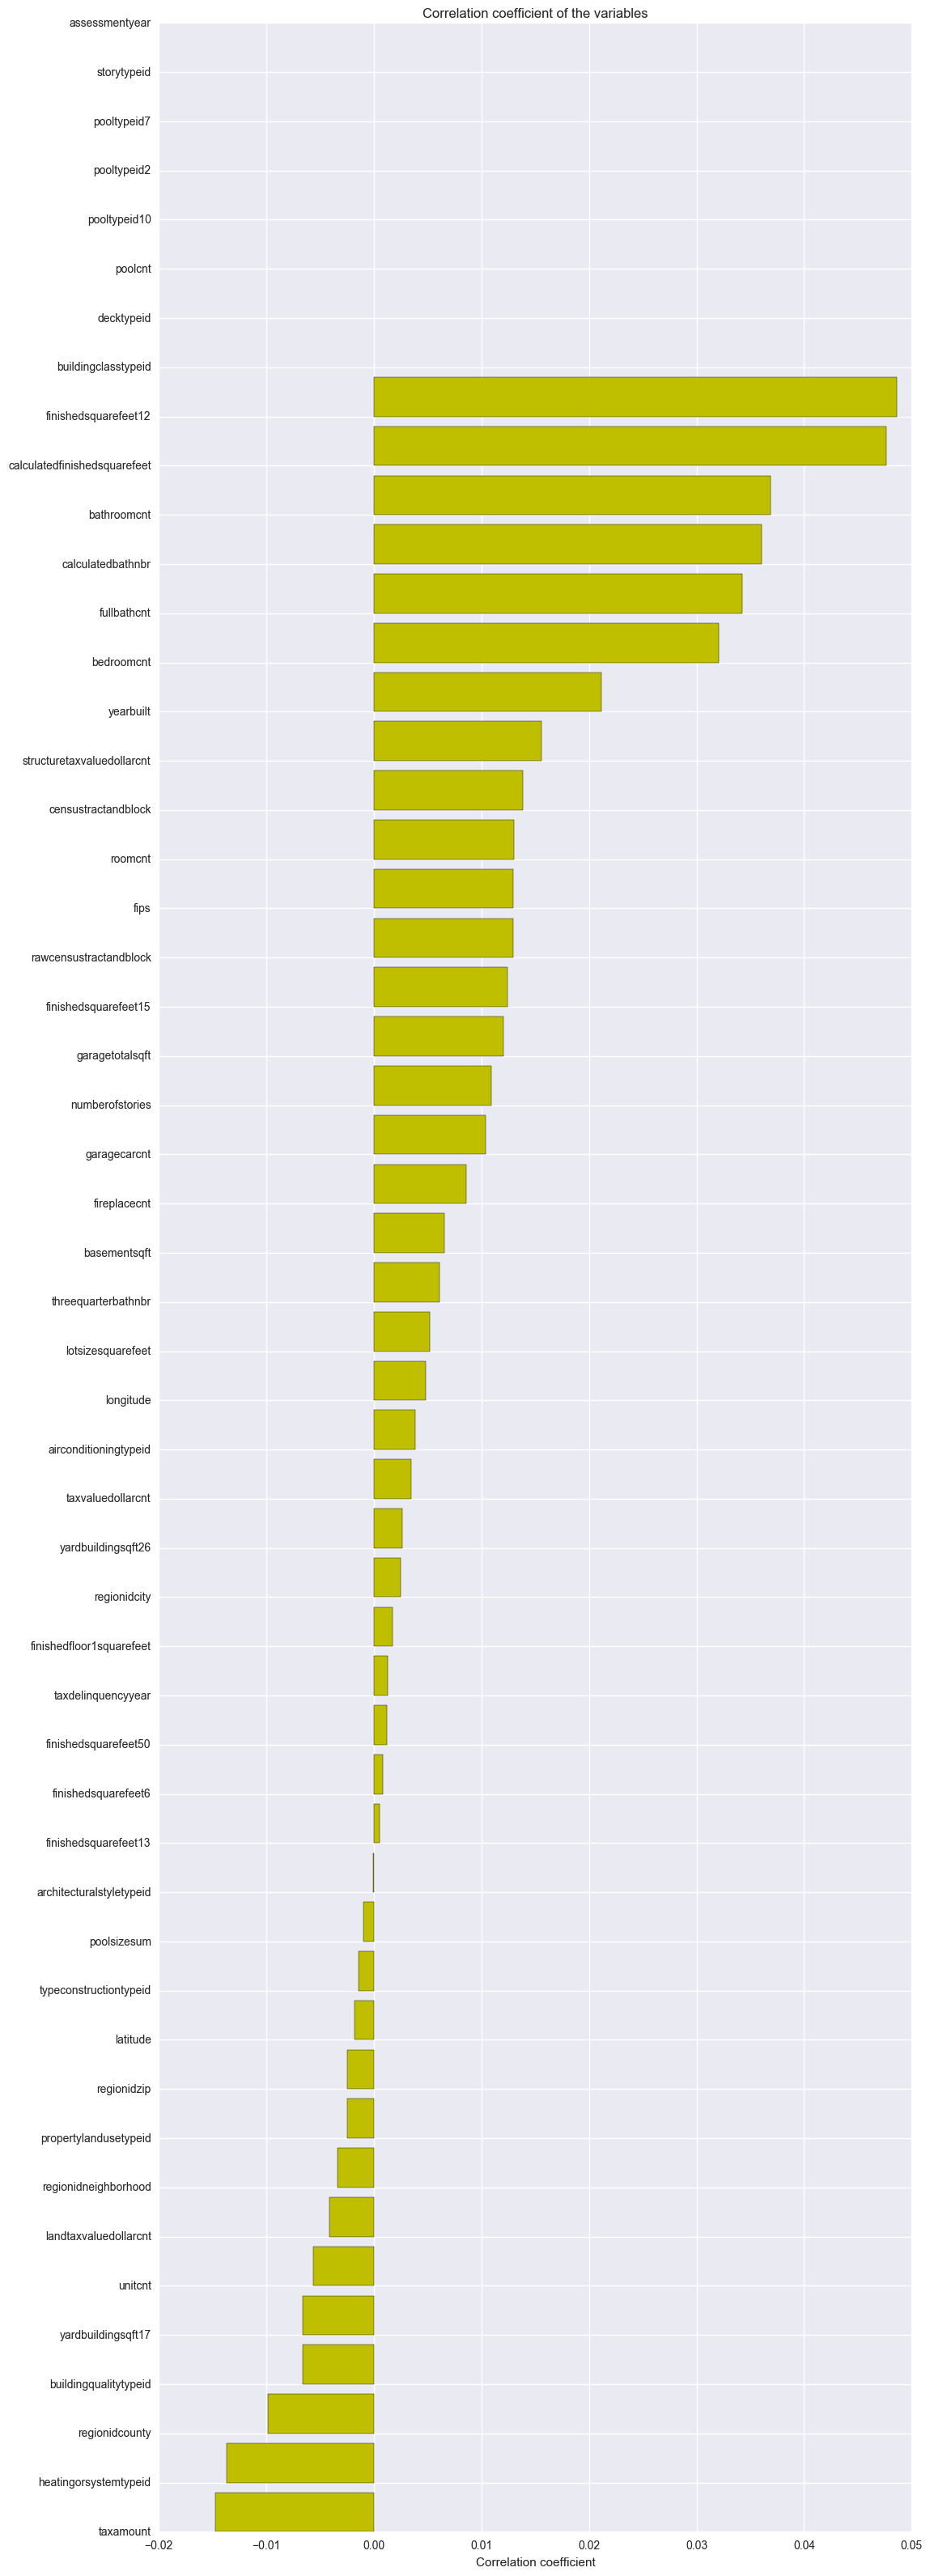
\includegraphics[width=0.6\textwidth]{./img/prop-important.png}
\caption{\label{fig:prop-important} Correlation between features and the log error}
\end{figure}
There are many features, so let take a look at the correlation between the logerror and these features to
see which ones seems to be more likely to improve the prediction than others.
Looking at Figure \ref{fig:prop-important} we can see
\begin{itemize}
    \item corrolation is low in general which indicate that improving prediction will be hard
    \item a few features are missing corrolation most likely because there are only one value
\end{itemize}

\begin{figure}
\centering
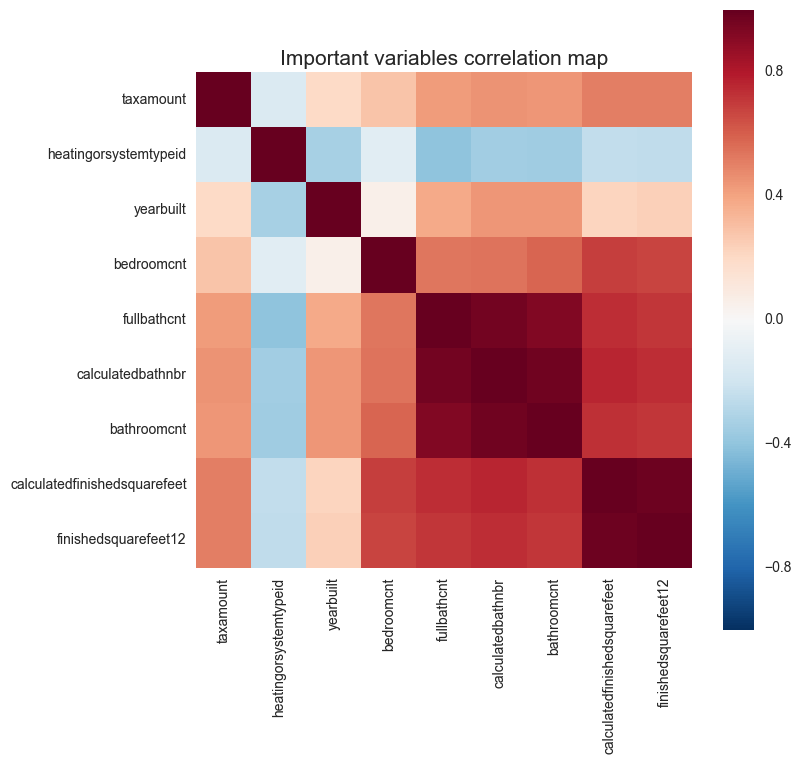
\includegraphics[width=1\textwidth]{./img/prop-corr-feature.png}
\caption{\label{fig:prop-corr-feature} Correlation between features and the log error}
\end{figure}
If we look at features with a corrolation less than -0.01 and more than 0.02 we may filter out nine features. High
corrolation between these featues might indicate that they contain the same type of information which most
likely makes prediction harder than if little correlation exists. Looking at Figure \ref{fig:prop-corr-feature}
show quite high correlation between features, especially between featues relating to room counts and house size.


\subsection{Algorithms and Techniques}
% Algorithms and techniques used in the project are thoroughly discussed and properly justified based on
% the characteristics of the problem.

% todo
% lista fördelar med LightGBM
% lista fördelar med Xgboost
% beskriv varför konstant modell är en enkel model och kan förbättra resultat
% beskriv varför det är bra att vikta resultatet

\subsection{Benchmark}
% Student clearly defines a benchmark result or threshold for comparing performances of solutions obtained.
The solution will be compared in two ways. First by splitting up the training data in file \textit{train\_2016.csv}
into a train and a test set. This will enable to test different models and configuration of models. Good candidates
can then be omited to the public leader board of Kaggle to be comapred towards other team models.

\section{Methodology}

\subsection{Data Preprocessing}
% All preprocessing steps have been clearly documented. Abnormalities or characteristics about the data or
% input that needed to be addressed have been corrected. If no data preprocessing is necessary, it has been
% clearly justified.
The data is prepared in following steps before feeded to LightGBM and Xgboost.
% TODO: replace with a ordered itemizer
\begin{itemize}
    \item Remove outliers to prevent the model to reduce generatalization due to data points not likely to
        reflect possible future data
    \item Convert types so that the data can be used in LightGBM and Xgboost
    \item Enriching the train data in file \textit{train\_2016.csv} with property data in file
        \textit{properties\_2016.csv} by joining on \textit{parcelid}
    \item Adding the month of the transaction as a feature
    \item Removed columns \textit{parcelid} and \textit{transactiondate} since these will most likely not
        improve the prediction
    \item Split data into train and test
\end{itemize}

\subsection{Implementation}
% The process for which metrics, algorithms, and techniques were implemented with the given datasets or input
% data has been thoroughly documented. Complications that occurred during the coding process are discussed.
The overall implementation steps are
% TODO: replace with a ordered itemizer
% TODO: get name for performance matric
\begin{itemize}
    \item Preprocessing and train for LightGBM using train data
    \item Preprocessing and train for Xgboost using train data
    \item Use linear regression to find the best weights on weighing together LightGBM, Xgboost, and the constant
        model using the train data
    \item Predict \textit{logerror} for test data using LightGBM
    \item Predict \textit{logerror} for test data using Xgboost
    \item Predict final \textit{logerror} for test data weighing weighing together LightGBM, Xgboost, and the
        constant model
    \item Compute the performance using the ?? matric
    \item Adjust configuration parameters for LightGBM and Xgboost and start over at the top
\end{itemize}


\subsection{Refinement}
% The process of improving upon the algorithms and techniques used is clearly documented. Both the initial and
% final solutions are reported, along with intermediate solutions, if necessary.

\section{Results}

\subsection{Model Evaluation and Validation}
% The final model’s qualities — such as parameters — are evaluated in detail. Some type of analysis is used
% to validate the robustness of the model’s solution.

\subsection{Justification}
% The final results are compared to the benchmark result or threshold with some type of statistical analysis.
% Justification is made as to whether the final model and solution is significant enough to have adequately
% solved the problem.

\section{Conclusion}

\subsection{Free-Form Visualization}
% A visualization has been provided that emphasizes an important quality about the project with thorough discussion.
% Visual cues are clearly defined.

\subsection{Reflection}
% Student adequately summarizes the end-to-end problem solution and discusses one or two particular aspects of
% the project they found interesting or difficult.

\subsection{Improvement}
% Discussion is made as to how one aspect of the implementation could be improved. Potential solutions resulting
% from these improvements are considered and compared/contrasted to the current solution.


\end{document}